\documentclass[a4paper, 12pt]{article}

\usepackage{graphicx}
\usepackage{float}
\usepackage[hidelinks=true]{hyperref}
\usepackage{amsmath}
\usepackage{amsfonts}

\author{Adrian Borup (adbo@itu.dk)}
\title{\textbf{The Leap Year Algorithm}}

\begin{document}
  \maketitle
  \section{A brief description of The Leap Year\\Algorithm}
  The Leap Year Algorithm is a simple algorithm to derive whether a year is a leap year. The algorithm can be applied to all numbers $y$ (representing a year) such that $y \in \{ n \in \mathbb{Z} \ | \ 1582 \leq n \}$.

  Let $P$ denote the predicate $4\,|\,y$, let $Q$ denote the predicate $100\,|\,y$, and let $S$ denote the predicate $400\,|\,y$. The algorithm states that $y$ is a leap year iff $(P \land \lnot Q) \lor S$.

  The accompanying software implementation of this algorithm follows the general flow diagram shown in \autoref{fig:flowdiagram} on page \pageref{fig:flowdiagram}. That is, once the input ``\textit{year}'' is received, the program shall check if \textit{year} abides by the constraints on $y$. If not, the program terminates early with an error---such as when \textit{year} is not an integer or the integer is outside the accepted range. If \textit{year} satisfies the constraints and $(P \land \lnot Q) \lor S$ is also true, the boolean \texttt{true} is returned. Otherwise, the boolean \texttt{false} is returned.

  \begin{figure}[H]
    \centering
    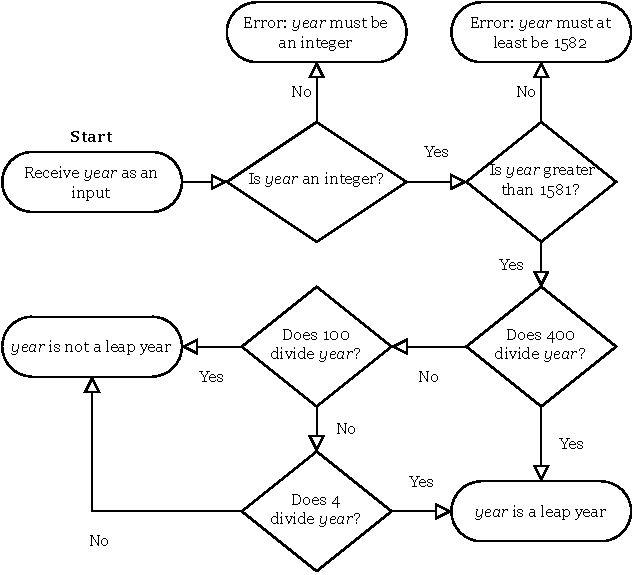
\includegraphics[width=1\textwidth]{assets/IsLeapYear_algorithm.pdf}
    \caption{A flow diagram illustrating the leap year algorithm.}
    \label{fig:flowdiagram}
  \end{figure}
  \vfill
  \noindent
  {\footnotesize Yes, I made the textual description overly complicated as a joke. Please do forgive me, for I had no idea what text to put upon this paper.}
\end{document}
